% Capitolo 3

\chapter{Un'architettura per la Rete Mocambos}
\label{Capitolo3}
\lhead{Capitolo 3. \emph{Un'architettura per la Rete Mocambos}}

\section{Specifica dei requisiti}
La Rete Mocambos attualmente è composta da piu di 200 comunità
localizzate in tutto il territorio nazionale brasiliano e alcune
comunità in Africa e in Europa. La connettività in Brasile è
satellitare, garantita dal programma GESAC che mette a disposizione di
ogni comunità un Very Small Aperture Terminal (VSAT) con banda di 512
kbit/s in download e 128 kbit/s in upload. La topologia della rete è a
stella per cui tutti i nodi comunicano tramite satellite concentrando
il traffico su un hub terrestre, dove la rete satellitare è
interconnessa a Internet. Ogni comunità ha a disposizione una sala con
10 computer ad accesso pubblico, installati recentemente tramite il
Telecentros.BR\footnote{``Il programma nazionale di appoggio
  all'inclusione digitale nelle comunità, Telecentros.BR, è un'azione
  del Governo Federale di appoggio per la creazione di nuovi spazi
  pubblici e comunitari di inclusione digitale e per il potenziamento
  degli spazi già in funzione su tutto il territorio. Vengono messe a
  disposizione le apparecchiature informatiche e il mobiliario
  necessario al funzionamento dei \textit{telecentros}, servizi di
  connessione a internet tramite banda larga oltre a formazione e
  borse per l'appoggio economico per tutor che lavorano come agenti di
  inclusione digitale. Questi tutor borsisti partecipano ad un corso
  di formazione e lavorano, nei telecentros, per le comunità.'',
  tradotto da \url{http://www.inclusaodigital.gov.br/telecentros}.},
altro programma federale brasiliano. La popolazione di ogni comunità
varia dalle centinaia alle migliaia di persone. La maggior parte delle
comunità si trova in area rurale, spesso di difficile accesso e priva
di altri mezzi di comunicazione. A parte gli spazi comunitari,
normalmente concentrati in una zona centrale, la popolazione è divisa
in piccoli nuclei familiari sparsi sul territorio e a volte molto
distanti tra di loro.

Vediamo alcuni requisiti essenziali per questa architettura di rete
federata.

\subsection{Identità di rete}
Gli utenti delle comunità devono avere associate delle identità
digitali con cui accedere e utilizzare i servizi esistenti. Oltre ad
accedere localmente, è importante avere accesso ad alcuni servizi
anche al di fuori della propria comunità. Ad esempio, nel caso una
persona si trovi in città, deve poter accedere, attraverso internet,
ai servizi base, quale l'email, o ai portali e servizi web della
RM. È necessaria quindi un identità digitale di rete univoca.

\subsection{Autenticazione decentrata}
\label{sec:AutDec}
Un requisito essenziale per ogni comunità è l'autonomia in assenza di
collegamento ad internet, e la presenza quindi di un sistema locale di
autenticazione e autorizzazione. Oltre a garantire la continuità del
servizio (in relazione a problemi di connessione satellitare), è un
requisito importante per un buon disimpegno di tutti i servizi
autenticati.

\subsection{Sincronizzazione}
Lo scambio di informazioni tra le comunità è l'obbiettivo primario per
la RM. È quindi necessario un meccanismo per la sincronizzazione
selettiva dei contenuti di interesse generale. Inoltre, per
ottimizzare l'uso della banda, le operazioni di sincronizzazione dei
dati devono incidere il meno possibile sull'uso quotidiano di internet,
programmando queste operazioni per la notte o comunque quando la
connessione satellitare non è utilizzata. Il sistema deve prevedere
anche la possibilità di sincronizzare i dati da e verso periferiche di
archiviazione di massa.

\subsection{Riproducibilità}
Ogni comunità provvede autonomamente alla gestione della propria infrastruttura
tecnologica e le soluzioni adottate devono quindi essere facilmente
implementabili e adattabili localmente. Gli strumenti devono quindi essere
soluzioni stabili e possibilmente di uso comune, anche al fine di
reperire piu facilmente assistenza in loco. 

\subsection{Manutenzione}
La manutenzione del sistema deve prevedere sia interventi a distanza
sia locali. Il sistema deve essere basato su tecnologie standard e
aperte per garantire l'accesso ai dati anche in caso di problemi.

\subsection{Sviluppo}
Ogni comunità ha caratteristiche e necessità proprie che portano alla
richiesta di servizi differenziati. L'architettura generale della RM
deve essere una base stabile su cui poter sviluppare servizi senza
vincoli troppo stringenti. Le tecnologie e i linguaggi adottati devono
facilitare l'interazione, la formazione e il riuso delle conoscenze. 

\section{Strumenti e pratiche per lo sviluppo}
Data la natura della RM, e in particolare la necessita di autonomia
tecnologica, la formazione è fondamentale per cui è importante l'uso
di strumenti che facilitino la documentazione e lo sviluppo
collettivo. La RM utilizza già da anni un wiki\footnote{``Una Wiki è
  una pagina (o comunque una collezione di documenti ipertestuali) che
  viene aggiornata dai suoi utilizzatori e i cui contenuti sono
  sviluppati in collaborazione da tutti coloro che vi hanno
  accesso. La modifica dei contenuti è aperta, nel senso che il testo
  può essere modificato da tutti gli utenti (a volte soltanto se
  registrati, altre volte anche anonimi) contribuendo non solo per
  aggiunte come accade solitamente nei forum, ma anche cambiando e
  cancellando ciò che hanno scritto gli autori precedenti.  Ogni
  modifica è registrata in una cronologia che permette in caso di
  necessità di riportare il testo alla versione precedente; lo scopo è
  quello di condividere, scambiare, immagazzinare e ottimizzare la
  conoscenza in modo collaborativo. Il termine wiki indica anche il
  software collaborativo utilizzato per creare il sito web e il
  server.'', tratto da \url{http://it.wikipedia.org/wiki/Wiki}.},
disponibile all'indirizzo \url{http://wiki.mocambos.net}, dove è
disponibile, in lingua portoghese, una parte della documentazione sul
codice sviluppato per questo lavoro. Per il versionamento del codice
del lavoro svolto si è scelto di usare il sistema decentrato GIT (vedi
\ref{sec:GIT}) e la piattaforma
GITHUB\footnote{\href{http://github.com}{GITHUB} è una rete sociale
  basata sul sistema GIT \ref{sec:GIT}.}. Il codice del prototipo è
disponibile all'indirizzo \url{https://github.com/RedeMocambos}

\subsection{Sistema operativo}
La scelta di un sistema operativo comune facilita la documentazione,
l'automazione e l'assistenza a distanza. Molte comunità utilizzano già
distribuzioni GNU/Linux basate su Debian\footnote{``Il Progetto Debian
  è una associazione di persone che ha come scopo comune la creazione
  di un sistema operativo libero. Il sistema operativo che abbiamo
  creato si chiama Debian GNU/Linux, o semplicemente Debian.'', tratto
  da \url{http://www.debian.org/}}. Per il prototipo sono state scelte
l'ultima versione stabile, di Debian, la 6.0, e di
Ubuntu\footnote{``Ubuntu è un sistema operativo GNU/Linux nato nel
  2004, basato su Debian, che si focalizza sull'utente e sulla
  facilità di utilizzo. Ubuntu è orientato all'utilizzo desktop e pone
  una grande attenzione al supporto hardware. È prevista una nuova
  versione ogni sei mesi.  Finanziato dalla società Canonical Ltd
  (registrata nell'Isola di Man), questo sistema è rilasciato come
  software libero sotto licenza GNU GPL ed è gratuito e liberamente
  modificabile.'', tratto da
  \url{http://it.wikipedia.org/wiki/Ubuntu}.}, la 11.10.

\subsection{Linguaggi di programmazione}
Per il sistema sviluppato si è scelto l'uso del linguaggio di
programmazione Python, un linguaggio molto flessibile e probabilmente
il più versatile per connettere componenti eterogenee. Inoltre alcune
comunità già usano Software Liberi, quali
\emph{GIMP}\footnote{\emph{GNU Image Manipulation Program (GIMP)} è un
  programma per il fotoritocco, montaggio e creazione di
  immagini. Disponibile su \url{http://www.gimp.org/}.},
\emph{Blender}\footnote{\emph{Blender} è un programma per la creazione
  di grafica e ambienti tridimensionali. Disponibile su
  \url{http://www.blender.org/}.},
\emph{Inkscape}\footnote{\emph{Inkscape} è un programma di grafica
  vettoriale conforme allo standard SVG. Disponibile su
  \url{http://inkscape.org}.} che fanno ampio uso di \emph{scripting}
Python per la creazione di filtri e per altre funzionalità avanzate.

\subsection{Virtualizzazione}
Il prototipo è stato sviluppato e testato in un ambiente
virtualizzato, per garantire maggior controllo e verificare la
correttezza del procedimento in tutti i suoi passaggi. Gli
\emph{script} per automatizzare le installazioni, e le procedure passo
passo presenti nella documentazione, sono state eseguite a partire da
un sistema base. Sono state create delle macchine virtuali, con
l'aiuto del programma libero
\emph{VirtualBox}\footnote{\emph{VirtualBox} è un virtualizzatore
  completo per architettura x86 per l'uso in server, computer
  personali e sistemi \emph{embedded}. Dispobibile su
  \url{http://www.virtualbox.org/}.}, simulando dei server
comunitari/locali e il server centrale.


\section{Architettura di base}

\subsection{Gestione delle identità di rete}
Analizzando la specifica dei requisiti e alcune delle tecnologie
esistenti viste nel capitolo precedente, è stato scelto l'uso di LDAP
per gestire le credenziali degli utenti all'interno della RM. Il
prototipo proposto prevede un server centrale su connettività internet
garantita e server locali in replica. È possibile pensare una
configurazione in cui tutti i server della rete sono configurati in
modalità N-Way-Multimaster. Questa configurazione, se da un lato
consente l'aggiornamento in scrittura della base utenti su ognuno dei
server, può generare più facilmente situazioni di inconsistenza dei
dati e problemi di sincronizzazione tra i server LDAP. Per questo
motivo per il prototipo realizzato si è scelto di rilassare il
requisito \ref{sec:AutDec}, ipotizzando un singolo server master per
tutta la rete su cui effettuare le operazioni in scrittura (creazione,
eliminazione e aggiornamento di utenti) e server locali abilitati solo
ad operazioni in lettura. Ogni comunità quindi avrebbe a disposizione
un server LDAP in replica su cui basare le operazioni di
autenticazione e autorizzazione. In mancanza di connessione esterna i
servizi locali rimangono comunque attivi per le utenze attive fino
all'ultima sincronizzazione.


\subsection{Mocambos\_LDAP}\label{MocambosLDAP}
\framebox[\textwidth]{\footnotesize Il codice è disponibile su
\url{https://github.com/RedeMocambos/Mocambos_LDAP}}

Per facilitare l'implementazione dei server LDAP dagli amministratori
locali è stato sviluppato uno script di installazione, che può tornare
utile anche per un amministratore remoto.

Lo script \textit{bash} provvede ad installare i pacchetti necessari e
preparare il server LDAP \emph{slapd} in configurazione master o
replica. Inoltre crea un DIT preconfigurato per la RM con una semplice
struttura (vedi figura \ref{fig:DIT_ReteMocambos}).

\begin{figure}[htbp]
  \centering
  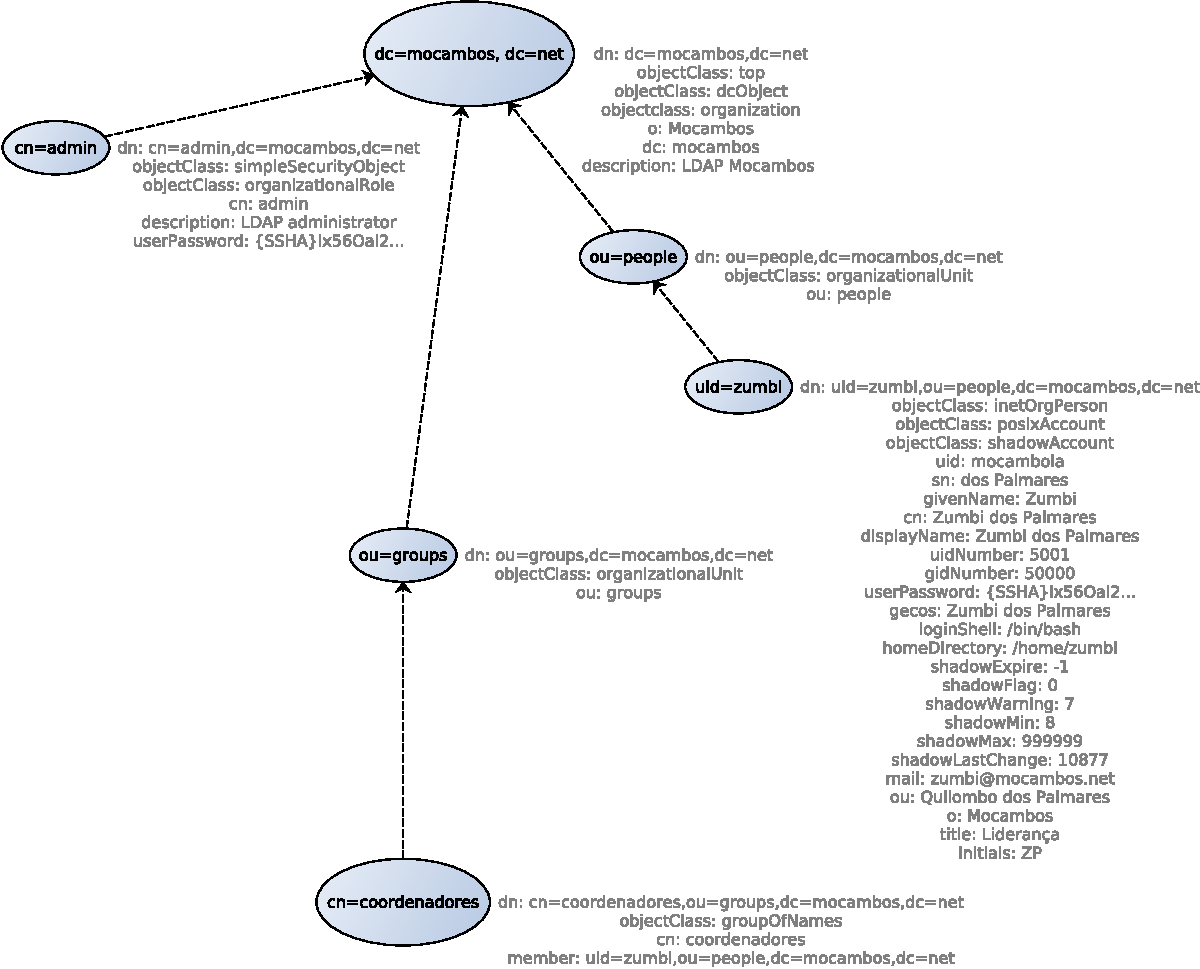
\includegraphics[width=\textwidth]{./Figure/DIT_ReteMocambos-crop.pdf}
  \rule{35em}{0.5pt}
  \caption[DIT di base del server LDAP della RM]{DIT di base del
    server LDAP della RM.}
  \label{fig:DIT_ReteMocambos}
\end{figure}




